\chapter{Background\markboth{Background}{}}

\section{Vehicle-to-Everything (V2X) Communication}

Vehicle-to-Everything (V2X) communication is a groundbreaking technology that enables vehicles to exchange data with
 their surroundings, including other vehicles, infrastructure, pedestrians, and cloud-based systems.
  This interconnected framework is a cornerstone of modern \ac{ITS}, designed to enhance road safety, improve traffic flow, and facilitate autonomous driving.

\subsection{Types of V2X Communication}
V2X encompasses several key components. \ac{V2V} communication allows direct data exchange between vehicles, 
enabling applications such as collision avoidance and coordinated lane changes. \ac{V2I} 
extends this interaction to roadside elements like traffic lights and road sensors, which provide vehicles with vital 
updates about traffic conditions or hazards. Additionally, \ac{V2P} communication ensures vehicles
 are aware of nearby pedestrians, even in scenarios with poor visibility. Finally, \ac{V2C} links vehicles 
 to cloud servers for updates on navigation, weather, or software improvements \cite{8605302}. 

 \begin{figure}[H]
    \centering
    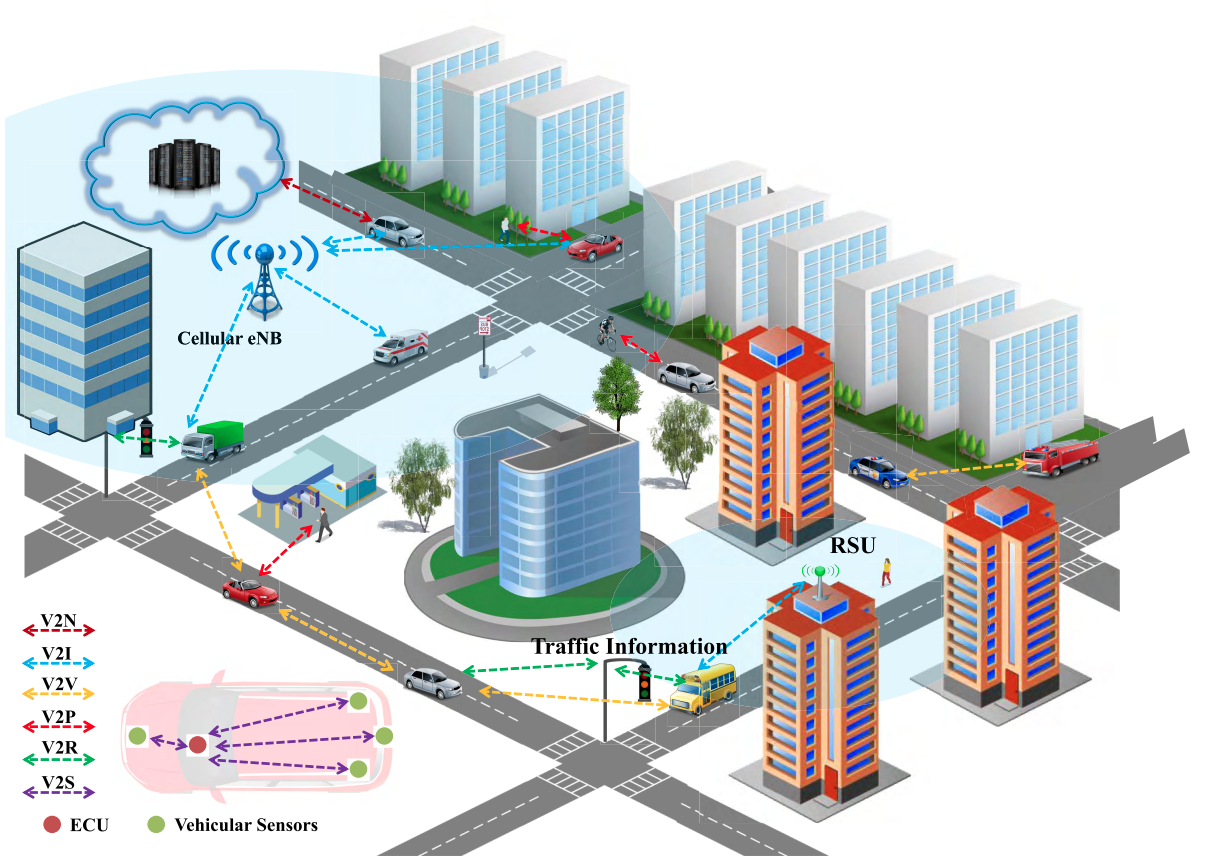
\includegraphics[width=1\textwidth]{images/figure1.png}
    \caption{An overview of V2X scenario}
    \label{fig:fig1}
\end{figure}

Figure~\ref{fig:fig1} illustrates a V2X communication network in a smart city environment, showcasing the interactions between
 vehicles, infrastructure, pedestrians, and networks. Various types of V2X communication are represented:
  \ac{V2N} connects vehicles to cloud-based systems via the Cellular \ac{eNB},
   which serves as the backbone of the cellular communication infrastructure. The Cellular eNB provides real-time updates
    and broad connectivity by leveraging 4G LTE and 5G technologies, enabling vehicles to access services such as navigation, 
    traffic information, and emergency alerts \cite{cite-key}. 

Vehicle-to-Infrastructure (V2I) is enabled through \ac{RSUs}, which are positioned near roadways 
and intersections. RSUs act as intermediaries between vehicles and the infrastructure, collecting and disseminating
 localized traffic information such as signal timings, road hazards, or construction updates. These units enhance 
 traffic management and safety by maintaining a continuous flow of communication with nearby vehicles and infrastructure 
 elements like traffic lights and road signs \cite{10806826}. 
    

 \subsection{Technologies Enabling V2X Communication}

 The technology behind V2X is built on two major standards. \ac{DSRC},
 a Wi-Fi-based protocol, is optimized for low-latency, reliable communication, making it suitable for 
 safety-critical applications like emergency braking. \ac{C-V2X}, on the other hand, leverages 
 4G LTE and 5G networks to support broader connectivity, enabling advanced functionalities such as real-time updates and 
 large-scale data sharing \cite{cite-key1}. 

 \subsection{Applications of V2X Communication}

Applications of V2X are vast and transformative. In addition to enhancing safety through 
collision prevention, V2X optimizes traffic management by reducing congestion and enabling 
efficient vehicle platooning. For autonomous vehicles, V2X complements onboard sensors like 
cameras and LiDAR, providing an additional layer of environmental awareness \cite{Sidorenko2024}. 

\subsection{Security Challenges in V2X Communication}

Despite its potential, V2X faces several challenges. Security and privacy concerns arise from the constant exchange 
of real-time data, while ensuring seamless interoperability across manufacturers remains a significant hurdle \cite{zEslami}.

A critical subset of V2X communication is the Vehicular Ad Hoc Network (VANET), which enables vehicles to form dynamic,
 self-organized communication networks without relying on fixed infrastructure. In VANETs, vehicles act as both transmitters
  and receivers, exchanging information with other vehicles (V2V) and infrastructure (V2I). The decentralized nature of VANET allows for real-time 
  communication, making it essential for time-sensitive applications. However, this decentralized architecture also 
  introduces unique security and privacy challenges.

The challenges of VANET stem primarily from the misuse of information provided by vehicles. Clearly, the use of
 incorrect messages can lead to accidents and the adoption of erroneous strategies by traffic control centers. 
 Therefore, the completeness and authenticity of messages must be verified before use \cite{zEslami}.

Additionally, one of the essential security requirements of VANET is conditional privacy preservation. 
Conditional privacy means that while others are unable to identify vehicles based on their transmitted messages, 
it should still be possible to trace vehicles if necessary. Furthermore, given the coverage 
limitations of RSUs and the traffic volume within these areas, data compression becomes a critical
 issue that must be addressed in VANET systems to maintain efficient communication \cite{zEslami}.